%! Author = eliainnocenti
%! Date = 04/10/23

% Preamble
\documentclass[11pt]{article}

% Packages
\usepackage{amsmath}
\usepackage{graphicx}
\usepackage{float}
\usepackage{listings}
\usepackage[font=small]{caption}
\usepackage{comment}
\usepackage[linesnumbered,vlined]{algorithm2e}
\usepackage{hhline}

% Images path
\graphicspath{ {./images/} }

% TODO - put a comment
\renewcommand{\contentsname}{Index}
\renewcommand{\figurename}{Figure}
\renewcommand{\tablename}{Table}

\SetAlgoCaptionSeparator{}

% Style % TODO - check
\lstdefinestyle{mystyle}{
    basicstyle=\ttfamily\footnotesize,
    breakatwhitespace=false,
    breaklines=true,
    captionpos=b,
    keepspaces=true,
    numbers=left,
    numbersep=5pt,
    showspaces=false,
    showstringspaces=false,
    showtabs=false,
    tabsize=2
}
\lstset{style=mystyle}

% Document intestation
\title{String Matching Algorithms \\
       \vspace{0.5em}
       \large Naive and KMP algorithms implementation and analysis}
\author{Elia Innocenti}
\date{November 2023}

    % Svolgere ed analizzare opportuni esperimenti
    % Scrivere una relazione (in LATEX) che descriva quanto fatto

    % deve contenere:
        % breve introduzione che descrive il problema
        % una breve descrizione delle caratteristiche teoriche degli algoritmi e delle strutture dati utilizzate
        % una valutazione a priori delle prestazioni attese degli algoritmi analizzati sperimentalmente
        % una descrizione degli esperimenti che verranno fatti (non un semplice elenco)
        % la documentazione del codice implementato
        % i risultati sperimentali, sia in tabelle che con grafici l’analisi completa di tali risultati, effettuata in modo critico

    % la teoria:
        % Fa riferimento a quanto studiato nel corso di Algoritmi e Strutture Dati
        % Deve essere solo la parte finalizzata all’esperimento
        % Non va bene un semplice copia/incolla dagli appunti (libro)
        % Bisogna descrivere gli aspetti più importanti e come questi indichino indirettamente quali test eseguire
        % Se serve un teorema, basta mostrarne l’applicazione non serve la dimostrazione

    % documentazione del codice:
        % uno schema del contenuto e delle interazioni fra i moduli uno schema delle classi
        % un’analisi delle scelte implementative effettuate
            % se erano possibili alternative, indicare perché è stata fatta una certa scelta
        % una descrizione dei metodi implementati, indicando in particolare l’input/output e la funzione svolta

    % descrizione degli esperimenti condotti:
        % Bisogna descrivere: i dati utilizzati
            % Se sono stati generato automaticamente, come questo avviene
            % Altrimenti da dove provengono e quali sono le loro caratteristiche
        % Specifiche della piattaforma di test (hardware, sistema operativo);
        % Quali misurazioni vengono effettuate
            % Che tipo di misure
            % Quante volte si eseguono i vari test
        % Come si effettuano le misurazioni (porzioni di codice osservate, numero di run effettuati)

    % presentazione risultati sperimentali:
        % Presentati sia in tabelle che con grafici
            % Le tabelle devono contenere tutti i dati (al limite in un file allegato)
            % I valori nelle tabelle devono avere un numero di cifre significative appropriato (python può fornire numeri con precisione arbitraria)
            % Un grafico serve per evidenziare l’andamento di un valore, ma non sostituisce la tabella
            % A volte possono essere presentati vari grafici per una tabella per mostrare aspetti diversi
            % Un grafico non chiaro o che non mostri qualcosa di interessante è inutile
            % Non importa la bellezza di un grafico
            % Tutti grafici le tabelle e le figure dvono essere
            % Descritti da una didascalia (lunga qb...)
            % Citati nel testo
            % \label{} ... \ref{}

    % analisi dei risultati sperimentali:
        % Un esperimento non è una semplice collezione di dati
        % I risultati di ogni esperimento vanno commentati ed analizzati in modo critico, citando i grafici e le tabelle corrispondenti
        % Nell’analisi si verifica se le ipotesi teoriche vengono verificate con i dati sperimentali
        % Al termine dell’analisi degli esperimenti un paragrafo di conclusioni è spesso utile per sintetizzare i risultati ottenuti

% Document
\begin{document}

    \maketitle
    \tableofcontents

    \newpage

    % Introduction
    \section{Introduction} \label{sec:introduction}

        In this report we would like to compare two algorithms for the \textbf{string-matching problem}, namely the \textbf{naive string-matching algorithm} and the \textbf{Knuth-Morris-Pratt algorithm}.

        \subsection{Hardware and software specifications} \label{subsec:hardware_software}

            Below are the specifications of the machine used to conduct the tests:
            \begin{itemize}
                \item \textbf{CPU:} Apple M1 SoC (System on Chip) with an 8-core CPU (4 high-performance and 4 high-efficiency cores), 7-core GPU, and Neural Engine
                \item \textbf{RAM:} 8GB unified memory
                \item \textbf{OS:} Sonoma 14.0
                \item \textbf{Python version:} 3.11
            \end{itemize}

    % The string matching problem
    \section{The string matching problem} \label{sec:string_matching_problem}

        \subsection{Definition} \label{subsec:definition}

            The \textbf{string-matching problem} is the problem of finding all occurrences of a pattern $P$ in a text $T$. \\

            We formalize the string-matching problem as follows. \\
            We assume that the test is an array $T[1..n]$ of length $n$ and that the pattern is an array $P[1..m]$ of length $m \leq n$ .
            We further assume that the elements of $T$ and $P$ are characters drawn from a finite alphabet $\Sigma$.
            For example, we may have $\Sigma = \{0, 1\}$ or $\Sigma = \{a, b, c, \dots, z\}$, the set of lowercase English letters.
            The character arrays $T$ and $P$ are often called strings of character. \\

            % FIXME - SOMETHING IS MISSING (shifts)

            The string-matching problem can also be seen as the problem of finding all valid shifts with which a given pattern $P$ occurs in a text $T$. \\

        \subsection{Example} \label{subsec:example}

            \begin{figure}[H]
                %\centering
                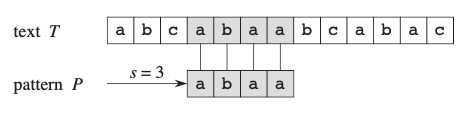
\includegraphics[width=0.5\textwidth]{Figure 2.1}
                \caption{An example of the string-matching problem.
                         Given the text $T = abcabaabcabac$ and the pattern $P = abaa$, we want to find all the occurrences of $P$ in $T$.
                         The pattern occurs only once in $T$, starting at shift $s = 3$.}
                \label{fig:example} % TODO - check label
            \end{figure}

            % TODO - align to the left (the system in the page and the equations in the system)
            \[
                \left\{
                \begin{aligned}
                    $0 \leq s \leq n - m$ \\
                    $T[s+1..s+m] = P[1..m]$ \\
                    $T[s+j] = P[j] for (1 \leq j \leq m)$ \\
                \end{aligned}
                \right.
            \]

        \subsection{Practical application} \label{subsec:practical_application}

            % TODO - check
            String matching algorithms have many practical applications in different fields:
            \begin{itemize}
                \item Text search: Find the occurrences of words or phrases within documents or long texts.
                \item Natural language processing: Analysing text to recognise language patterns, lexical analysis and parsing of texts.
                \item Computational biology: Analysing DNA, RNA and protein sequences to identify biological patterns and correlations.
                \item Log and structured text analysis: Recognise patterns in large datasets, such as system logs, sensor records, etc.
                \item Data filtering and analysis: They allow information to be extracted from large volumes of structured and unstructured data.
                \item Search engines: Working behind the scenes to identify the most relevant matches between user search queries and content.
                \item Data compression: Used in compression algorithms to find and replace repeated patterns.
                \item Computer security: Identify signatures and patterns of attacks by detecting byte sequences or malicious behaviour in data.
            \end{itemize}

    % The naive string-matching algorithm
    \section{The naive string-matching algorithm} \label{sec:naive_string_matching_algorithm}

        The naive algorithm finds all valid shifts using a loop that checks the condition $P[1..m] = T[s+1..s+m]$ for each of the $n - m + 1$ values of $s$.

        \subsection{Description} \label{subsec:naive_description}

            % TODO - REWRITE THE SECTION
            The naive string-matching algorithm proceeds sliding a ``template'' containing the pattern over the text, noting for which shifts
            all of the characters in the template match the corresponding characters in the text. \\
            The for loop consider each possible shift explicitly, and the if-condition implicitly loops to check corresponding characters
            position until all position match successfully or until a mismatch is found.

        \subsection{Pseudocode} \label{subsec:naive_pseudocode}

            % Naive algorithm pseudocode
            \SetAlgorithmName{}{naive_string_matching_algorithm}{}
            \begin{algorithm}[H] \label{alg:naive_string_matching_algorithm}
                \SetAlgoLined
                \KwData{Text $T$ of size $n$ and pattern $P$ of size $m$}
                \KwResult{All valid shifts with which $P$ occurs in $T$}
                \vspace{0.5em}
                \captionabove{\underline{NAIVE-STRING-MATCHER(T,P)}} \\
                \vspace{0.5em}

                    $n$ \leftarrow T.length\; \\
                    $m$ \leftarrow P.length\; \\
                    \For{$s \leftarrow 0$ \KwTo $n - m$}{
                        \If{$P[1..m] = T[s+1..s+m]$}{
                            print "Pattern occurs with shift" $s$\;
                        }
                    }

            \end{algorithm}

        \subsection{Time complexity} \label{subsec:naive_time_complexity}

            % FIXME - THIS IS NOT VALID
            % TODO - REWRITE THE SECTION
            The worst-case running time of the naive string-matching algorithm is $\Theta((n - m + 1)m)$, which is $\Theta(nm)$.
            The worst case occurs when the first $m - 1$ characters of the pattern match the first $m - 1$ characters of the text, but the last characters do not match.
            In this case, the algorithm performs $n - m + 1$ comparisons, each requiring $m$ character comparisons. \\

            The best-case running time of the naive string-matching algorithm is $\Theta(n)$.
            The best case occurs when the first character of the pattern does not occur in the text.
            In this case, the algorithm performs $n - m + 1$ comparisons, each requiring $1$ character comparison. \\

            The average-case running time of the naive string-matching algorithm is $\Theta(n)$.
            The average case occurs when the pattern does not occur in the text.
            In this case, the algorithm performs $n - m + 1$ comparisons, each requiring $m$ character comparisons.

    % String matching with finite automata
    \section{String matching with finite automata} \label{sec:string_matching_with_finite_automata}

        % TODO - REWRITE THE SECTION
        Some algorithms implement a finite automata - a simple machine for processing information - that scans the text string $T$ for all occurrences of the pattern $P$.
        These string-matching automata examine each text character exactly once, taking constant time per text character.
        The matching time used - after preprocessing the pattern to build the automaton - is therefore $\Theta(n)$, where $n$ is the length of the text.
        The time to build the automaton can be large if $\Sigma$ is large.

        \subsection{Finite automata}\label{subsec:finite_automata}

            Finite automata

    % The Knuth-Morris-Pratt algorithm
    \section{Knuth-Morris-Pratt algorithm} \label{sec:knuth_morris_pratt_algorithm}

        % TODO - REWRITE THE SECTION
        % TODO - CONNECT THE IDEA OF THE AUTOMATON TO THE KMP ALGORITHM
        The Knuth-Morris-Pratt algorithm improves the running time of the naive algorithm by using information about the pattern itself to avoid some comparisons.
        The key idea is that when a mismatch occurs, the pattern itself contains enough information to determine where the next match could begin, thus bypassing re-examination of previously matched characters.

        \subsection{Description}\label{subsec:kmp_description}

            Description

        \subsection{Pseudocode} \label{subsec:kmp_pseudocode}

            % KMP algorithm pseudocode
            \SetAlgorithmName{}{kmp_string_matching_algorithm}{}
            \begin{algorithm}[H] \label{alg:kmp_string_matching_algorithm}
                \SetAlgoLined
                \KwData{Text $T$ of size $n$ and pattern $P$ of size $m$}
                \KwResult{All valid shifts with which $P$ occurs in $T$}
                \vspace{0.5em}
                \captionabove{\underline{KMP-MATCHER(T,P)}} \\
                \vspace{0.5em}

                    $n$ \leftarrow T.length\; \\
                    $m$ \leftarrow P.length\; \\
                    \pi \leftarrow \text{COMPUTE-PREFIX-FUNCTION(P)}\; \\
                    $q$ \leftarrow $0$\; \\
                    \For{$i \leftarrow 1$ \KwTo $n$}{
                        \While{$q > 0$ and $P[q+1] \neq T[i]$}{
                            $q \leftarrow \pi[q]$\;
                        }
                        \If{$P[q+1] = T[i]$}{
                            $q \leftarrow q + 1$\;
                        }
                        \If{$q = m$}{
                            print "Pattern occurs with shift" $i - m$\;
                            $q \leftarrow \pi[q]$\;
                        }
                    }

            \end{algorithm}

            \vspace{0.0em}

            % Compute prefix function pseudocode
            \SetAlgorithmName{}{kmp_string_matching_algorithm}{}
            \begin{algorithm}[H] \label{alg:compute_prefix_function}
                \SetAlgoLined
                \KwData{Pattern $P$ of size $m$}
                \KwResult{Prefix function $\pi$}
                \vspace{0.5em}
                \captionabove{\underline{COMPUTE-PREFIX-FUNCTION(P)}} \\
                \vspace{0.5em}

                    $m$ \leftarrow P.length\; \\
                    let $\pi[1..m]$ be a new array\; \\
                    $\pi[1] \leftarrow 0$\; \\
                    $k \leftarrow 0$\; \\
                    \For{$q \leftarrow 2$ \KwTo $m$}{
                        \While{$k > 0$ and $P[k+1] \neq P[q]$}{
                            $k \leftarrow \pi[k]$\;
                        }
                        \If{$P[k+1] = P[q]$}{
                            $k \leftarrow k + 1$\;
                        }
                        $\pi[q] \leftarrow k$\;
                    }
                    \Return $\pi$\;

            \end{algorithm}

        \subsection{Time complexity} \label{subsec:kmp_time_complexity}

            % FIXME - THIS IS NOT VALID
            % TODO - REWRITE THE SECTION
            The worst-case running time of the Knuth-Morris-Pratt algorithm is $\Theta(n)$.
            The worst case occurs when the first character of the pattern does not occur in the text.
            In this case, the algorithm performs $n$ comparisons, each requiring $1$ character comparison. \\

            The best-case running time of the Knuth-Morris-Pratt algorithm is $\Theta(n)$.
            The best case occurs when the pattern does not occur in the text.
            In this case, the algorithm performs $n$ comparisons, each requiring $1$ character comparison. \\

            The average-case running time of the Knuth-Morris-Pratt algorithm is $\Theta(n)$.
            The average case occurs when the pattern does not occur in the text.
            In this case, the algorithm performs $n$ comparisons, each requiring $1$ character comparison.

    % Differences between naive string-matching and KMP algorithms
    \section{Differences between naive string-matching and KMP algorithms} \label{sec:naive_kmp_differences}

        \subsection{Preprocessing} \label{subsec:preprocessing}

            Preprocessing

        \subsection{Time complexity} \label{subsec:naive_kmp_time_complexity}

            % FIXME - TO BE FIXED (aesthetically)
            \begin{table}[H]
                \centering
                \resizebox{\textwidth}{!}{
                    \begin{tabular}{|c|c|c|c|c|}
                        \hhline{~~|---|}
                        \multicolumn{1}{c}{} & \multicolumn{1}{c|}{} & \multicolumn{3}{c|}{\textbf{Matching time}} \\
                        \hline
                        \textbf{Algorithm} & \textbf{Preprocessing time} & \textbf{Worst-case} & \textbf{Best-case} & \textbf{Average-case} \\
                        \hline
                        Naive & {$0$} & $\Theta((n-m+1)m)$ & $O((n-m+1)m)$ & $O((n-m+1)m)$ \\
                        \hline
                        KMP & {$\Theta(m)$} & $\Theta(n)$ & $\Theta(n)$ & $\Theta(n)$ \\
                        \hline
                    \end{tabular}
                }
                \caption{Time complexity of the naive and KMP algorithms.}
                \label{tab:naive_kmp_time_complexity}
            \end{table}

    % Tests and results
    \section{Tests and results} \label{sec:tests_and_results}

        Tests and results

        \subsection{Expected performances} \label{subsec:expected_performances}

            Expected performances

    % Conclusions
    \section{Conclusions} \label{sec:conclusions}

        Conclusions

\end{document}